%!TEX root = ../main.tex
%%%%%%%%%%%%%%%%%%%%%%%%%%%%%%%%%%
% Links:
%
% Difficulty: Companies: 
%%%%%%%%%%%%%%%%%%%%%%%%%%%%%%%%%%


%\begin{figure} \centering
%   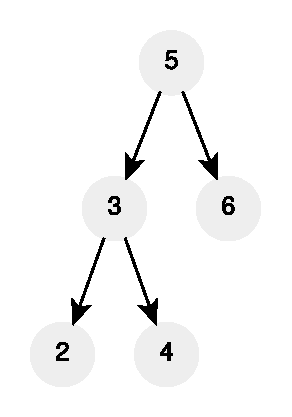
\includegraphics[width=\textwidth]{sources/remove_all_occurrences_unsorted_array_inplace/images/example1}
%   \caption[Sample short cpation]{Sample Caption}.
%   \label{fig:remove_all_occurrences_unsorted_array_inplace:example1} \end{figure}

\chapter{Remove all occurrences -  unsorted array}
\label{ch:remove_all_occurrences_unsorted_array_inplace}
\section*{Introduction}
The problem described in this chapter asks you to implement a common operations: removes all
elements satisfying specific criteria from a collection. This problem has lot of similarities with
the one described in Chapter \ref{ch:remove_duplicated_sorted_array_inplace} and as a consequence
they share the same general solution approach. 

There are many versions and variations of this problem with the most common being the one where the
collection is a simple array or a vector of integers and you are asked to remove all the elements
equal to a given integer. However here, we will discuss a more general version of this problem where
the collection is of a generic type \inline{T} and the criteria is given in the form of a unary
function returning a boolean\footnote{This type of functions is also commonly known as
\textit{predicate}.}. Specializing what is discussed here on the fly during the interview for the
actual particular problem's version given to you should be easy.


\section{Problem statement}
\begin{exercise}
\label{example:remove_all_occurrences_unsorted_array_inplace:exercice1}
Write a function that given a collection $I$ of elements of type \inline{T} and a predicate function
 $p$ with signature \inline{bool(const T&)}, rearranges $I$ in such a way that all the $0 \leq k
 \leq |I|$ elements satisfying $p$ in $I$ are moved to its front. The function should returns $k$.

 Moreover, the relative order of the elements  satisfying $p$ should be preserved: If both elements
 at indices $n$ and $m$ satisfy the predicate $p$  and $I_n$ comes before $I_m$ then when the
 function returns, their relative order is unchanged albeit they both might be moved to new
 locations.
 
	%example1
	\begin{example}
		\label{example:remove_all_occurrences_unsorted_array_inplace:example1}
		\hfill \\
		Given $I = \{[4, 1, 1, 2, 1, 3]\}$ and $p$ is a function returning true if its input
		argument is an even number, the function returns $4$. The first $4$ elements of $I$ are
		$\{1,1,1,3\}$. 
		
	\end{example}

	\begin{example}
		\label{example:remove_all_occurrences_unsorted_array_inplace:example2}
		\hfill \\
		Given $I = \{[4, 1, 1, 2, 1, 3]\}$ and $p$ is a function returning true if its input
		argument is odd, the function returns $2$. At this point, the first $2$ elements of $I$ are
		$\{4,2\}$. 
		
	\end{example}
\end{exercise}

\section{Clarification Questions}

\begin{QandA}
	\item What should be the content of $I$ from index $k+1$ and after?
	\begin{answered}
		\textit{There are no constraints on the content of those cells of $I$.}
	\end{answered}
	
\end{QandA}

\section{Discussion}
\label{remove_all_occurrences_unsorted_array_inplace:sec:discussion}
This problem could be restated as: \textit{Implement the
\inline{remove_if}\footnote{\url{https://en.cppreference.com/w/cpp/algorithm/remove}}} function from
the C++ STL. So I would not be really surprised if during an interview someone would come-up with a
one-liner as the one shown in Listing \ref{list:remove_all_occurrences_unsorted_array_inplace:STL}.
\footnote{Notice the similarities with Listing \ref{list:remove_duplicated_sorted_array_inplace_stl} for the problem in Chapter \ref{ch:remove_duplicated_sorted_array_inplace}}.
However, if you present this solution to the interviewer you might expect that he asks you to implement the logic behind \inline{std::remove_if}.

\lstinputlisting[language=c++, caption={One-liner solution using the STL functions \inline{distance} and \inline{remove_if}},label=list:remove_all_occurrences_unsorted_array_inplace:STL]{sources/remove_all_occurrences_unsorted_array_inplace/remove_all_occurrences_unsorted_array_inplace_solution1.cpp}


\subsection{Linear space}
\label{remove_all_occurrences_unsorted_array_inplace:sec:bruteforce}
There is a straightforward way of solving this problem that has also the additional benefit of occupy only a couple of lines and of being 
super clear and simple. The idea is that we can use an additional linear amount of space to temporarily store the valid (dissatisfying $p$) elements, and
in a subsequent phase move them into the front of $I$. Listing \ref{list:remove_all_occurrences_unsorted_array_inplace:copy} shows a possible implementation of this idea.
This solution however only works correctly for types that can be copied. The interviewer could well ask you to fix this and in that case you can 
loop over \inline{A} and \inline{temp} and \inline{move}\footnote{\url{https://en.cppreference.com/w/cpp/utility/move}} the elements around instead.
\lstinputlisting[language=c++, caption={Linear space solution using the \inline{std::copy} family of functions from the STL.},label=list:remove_all_occurrences_unsorted_array_inplace:copy]{sources/remove_all_occurrences_unsorted_array_inplace/remove_all_occurrences_unsorted_array_inplace_solution2.cpp}

\subsection{Constant space}
\label{remove_all_occurrences_unsorted_array_inplace:sec:constant_space}
The idea discussed in Section \ref{remove_all_occurrences_unsorted_array_inplace:sec:bruteforce} can quite easily be modified so that we avoid using linear
additional space. We could use move the elements of $A$ into $A$ itself, pretty much in the same fashion we already did for the problem discussed in Chapter \ref{ch:remove_duplicated_sorted_array_inplace}
while discussing the solution \ref{list:remove_duplicated_sorted_array_inplace}. 
We use exactly the same approach of two pointers $x$ and $y$ pointing to:
\begin{enumerate}
	\item $x$, keeping track of the new front to $I$. It points to the end of the portion of $I$ (starting at index $0$ and ending at $x-1$) containing all the valid elements found so far.
	\item $y$, which is a pointer to the next element not yet processed in $I$.
\end{enumerate}.
Listing \ref{list:remove_all_occurrences_unsorted_array_inplace:constant_space} implements this idea.

At the beginning of the execution the algorithm moves $x$ forward so that all the valid elements that are already
at the front of $I$ stay untouched where they are as they are already in the right locations.
At this point $x$ points either to the first invalid element in $I$ or to one element past $I$.
In the second scenario there is no more work to do. All the elements are valid to begin with and the second \inline{while}
will not even start. $I$ is left unchanged.
In the first scenario we will use $y$ to scan the remaining element of $I$ past $x$, and we move each valid element we encounter, 
into the location pointed by $x$. When this happen $x$ is moved forward as the portion of valid elements grew by one element. 

Notice that the invariant $x \leq y$ is always respected as:
\begin{itemize}
	\item it holds before the beginning of the loop and,
	\item $x$ is incremented at the same rate or less compare to $y$.
\end{itemize}
At the end of this process we are left with $y$ pointing to the one element past $I$ and $x$ pointing one cell after the last valid element of the newly rearranged $I$.

\lstinputlisting[language=c++, caption={Constant space solution using a two pointer approach.},label=list:remove_all_occurrences_unsorted_array_inplace:constant_space]{sources/remove_all_occurrences_unsorted_array_inplace/remove_all_occurrences_unsorted_array_inplace_solution3.cpp}


